
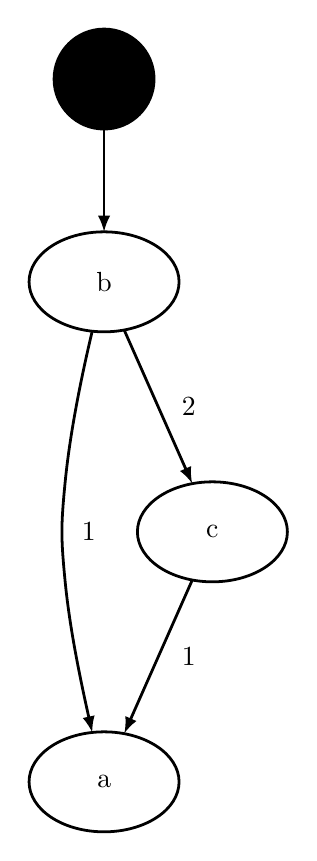
\begin{tikzpicture}[>=latex,line join=bevel,]
  \pgfsetlinewidth{1bp}
%%
\pgfsetcolor{black}
  % Edge: b -> a
  \draw [->] (22.729bp,180.21bp) .. controls (19.323bp,165.91bp) and (14.832bp,144.76bp)  .. (13bp,126bp) .. controls (11.445bp,110.08bp) and (11.445bp,105.92bp)  .. (13bp,90bp) .. controls (14.445bp,75.2bp) and (17.547bp,58.908bp)  .. (22.729bp,35.791bp);
  \definecolor{strokecol}{rgb}{0.0,0.0,0.0};
  \pgfsetstrokecolor{strokecol}
  \draw (21.5bp,108bp) node {1};
  % Edge: c -> a
  \draw [->] (58.664bp,90.448bp) .. controls (52.999bp,77.665bp) and (45.053bp,59.735bp)  .. (34.303bp,35.478bp);
  \draw (57.5bp,63bp) node {1};
  % Edge: b -> c
  \draw [->] (34.336bp,180.45bp) .. controls (40.001bp,167.66bp) and (47.947bp,149.74bp)  .. (58.697bp,125.48bp);
  \draw (57.5bp,153bp) node {2};
  % Edge: 0 -> b
  \draw [->] (27bp,252.81bp) .. controls (27bp,244.79bp) and (27bp,235.05bp)  .. (27bp,216.03bp);
  % Node: a
\begin{scope}
  \definecolor{strokecol}{rgb}{0.0,0.0,0.0};
  \pgfsetstrokecolor{strokecol}
  \draw (27bp,18bp) ellipse (27bp and 18bp);
  \draw (27bp,18bp) node {a};
\end{scope}
  % Node: 0
\begin{scope}
  \definecolor{strokecol}{rgb}{0.0,0.0,0.0};
  \pgfsetstrokecolor{strokecol}
  \definecolor{fillcol}{rgb}{0.0,0.0,0.0};
  \pgfsetfillcolor{fillcol}
  \filldraw [opacity=1] (27bp,271bp) ellipse (18bp and 18bp);
\end{scope}
  % Node: c
\begin{scope}
  \definecolor{strokecol}{rgb}{0.0,0.0,0.0};
  \pgfsetstrokecolor{strokecol}
  \draw (66bp,108bp) ellipse (27bp and 18bp);
  \draw (66bp,108bp) node {c};
\end{scope}
  % Node: b
\begin{scope}
  \definecolor{strokecol}{rgb}{0.0,0.0,0.0};
  \pgfsetstrokecolor{strokecol}
  \draw (27bp,198bp) ellipse (27bp and 18bp);
  \draw (27bp,198bp) node {b};
\end{scope}
%
\end{tikzpicture}

